\begin{figure}[H]
\centering
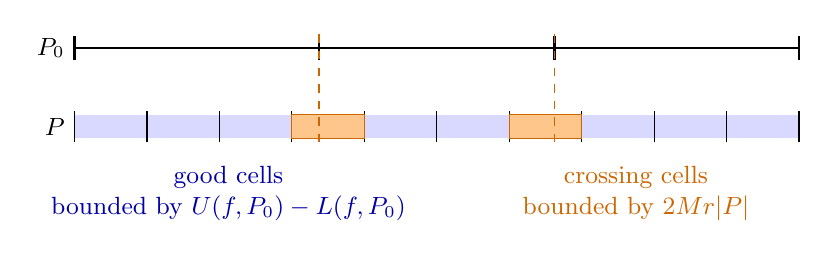
\begin{tikzpicture}[x=1.15cm,y=1cm,font=\small]
\node[left] at (0,1) {$P_0$};
\node[left] at (0,0) {$P$};
\draw[thick] (0,1)--(8,1);
\foreach \x in {0,2.7,5.3,8}{\draw[thick] (\x,.85)--(\x,1.15);}
\foreach \i in {0,...,9}{
\pgfmathsetmacro{\a}{.8*\i}
\pgfmathsetmacro{\b}{\a+.8}
\filldraw[fill=blue!15,draw=white] (\a,-.15) rectangle (\b,.15);
\draw (\a,-.2)--(\a,.2);
}
\foreach \a/\b in {2.4/3.2,4.8/5.6}{
\filldraw[fill=orange!45,draw=orange!80!black] (\a,-.15) rectangle (\b,.15);}
\draw (8,-.2)--(8,.2);
\foreach \x in {2.7,5.3}{\draw[dashed,orange!80!black] (\x,-.2)--(\x,1.25);}
\node[blue!65!black,align=center] at (1.7,-.85) {good cells\\bounded by $U(f,P_0)-L(f,P_0)$};
\node[orange!80!black,align=center] at (6.2,-.85) {crossing cells\\bounded by $2Mr|P|$};
\end{tikzpicture}
\caption{A fine partition need not refine the coarse one. Blue cells inherit
the coarse oscillation bounds; orange cells cross old division points.
Their total width is at most $r|P|$, so their gap contribution is at most
$2Mr|P|$.}
\label{fig:fine-crossing}
\end{figure}
